\section{Specific Requirements}
This section is devoted to a specific description of every kind of requirement the system has to deal with in order to achieve all the functionalities described.
\subsection{External interface Requirements}
\subsubsection{User Interfaces}
DREAM is divided into sections that could be accessed by the users of the system. Below there is the list of the section and the user that can access the section. When there are two divisions in the users it means that the section is the same, but it will show different functionalities.\\
\newline
\textbf{LogIn}\\
Login is the first page that opens each time any user opens DREAM. After typing the credentials given by Telangana’s state, the user has to click the “Log In” button to verify his/her credentials.\\
\newline
\textbf{Report a Problem}\\
Report a Problem allows farmers to report every problem they encounter during their activity. It also allows agronomists and TPM to visualize the farmer’s reported problems, either to prepare for the visits or to record the most common issues.\\
\newline
\textbf{WikiFarm}\\
WikiFarm is used by farmers and agronomists. After the user provides his/her zone and type of production, the system shows a list of the suggested crops and a list of the suggested fertilizers.\\
\newline
\textbf{Weather}\\
Weather is used by farmers and agronomists to visualize weather forecasts. The user has to provide his/her zone and a timeslot to visualize, then the system retrieves and shows the requested forecast.\\
\newline
\textbf{Report Production}\\
Report Production is used by farmers at the end of each month to report their production. It allows the farmers to insert data about each of their cultivation, then the system retrieves the data about soil humidity and water usage from the sensors and a complete report is published. The page can also be accessed by agronomists and TPM, to visualize the reports published by the farmers.\\
\newline
\textbf{Help}\\
Help is used by farmers to post help requests, which can be answered by other farmers and agronomists. To publish a new help request a farmer has to provide a description of his/her problem.\\
\newline
\textbf{Forum}\\
Forum allows farmers to create new discussions and reply to existing ones. In order to create a new discussion, a farmer has to insert a title and the topic of the discussion.\\
\newline
\textbf{Agenda}\\
Agenda is used by agronomists to visualize, change, and confirm their daily plan. It allows agronomists to open an event, either to visualize it, postpone it or publish a report after the visit is completed.\\
\newline
\textbf{Visualize Initiatives}\\
Visualize Initiatives allows TPM to visualize the reports associated to a farmer, in order to look at the initiatives taken by the agronomists who visited them. This is used by TPM to find the steering initiatives.\\
\newline
\textbf{Rankings}\\
Rankings is used by agronomists and TPM to create a ranking of the farmer’s performances in a zone. If the selected zone is “All”, the system will create a ranking of every farmer registered in DREAM.\\
\newline
\textbf{Chat}\\
Chat can be accessed by every user in order to create a new chat or reply to an open one. To create a new chat a user has to insert the username associated to the user he/she wants to contact.
\subsubsection{Hardware Interfaces}
To operate properly DREAM needs information about water usage and soil humidity of every farm, so two hardware components shall be provided to each farmer:
\begin{itemize}
    \item A humidity sensor, installed on the farm ground of every farmer
    \item A sensor to measure the water supplied to each farm through the water irrigation system
\end{itemize}
Furthermore, to access DREAM any user is required to own a device connected to internet.
\subsubsection{Software Interfaces}
The system interfaces with external IT providers in order to acquire the weather forecasts and to combine the information acquired by each farmer.
\subsubsection{Communication Interfaces}
All the communications from and to DREAM are made through the HTTPS protocol.

\newpage
\subsection{Use Cases Description}
Use cases capture functional requirements of a system from the users’ perspective.

%TODO: sistemare le dimensioni delle foto


\begin{table}[H]
    \centering
    \begin{tabular}{@{}p{0.25\linewidth}p{0.71\linewidth}@{}}
        \hline
        \textbf{Name} & Platform login \\
        \hline
        \textbf{ID} & \usecaseindex{UC.1} ~\\
        \hline
        \textbf{Actors} & TPM, Farmer, Agronomist \\
        \hline
        \textbf{Entry conditions} &
        \begin{itemize}[leftmargin=.4cm,noitemsep,topsep=0pt,before=\vspace{-3mm},after=\vspace{-4mm}]
            \item The platform is running
            \item The user is running the application on his/her device
        \end{itemize} \\
        \hline
        \textbf{Flow of events} &
        \begin{enumerate}[label=\roman*.,leftmargin=.5cm,noitemsep,topsep=0pt,before=\vspace{-3mm},after=\vspace{-4mm}]
            \item The user opens DREAM
            \item The user inserts their username and password
            \item The user clicks on “Log In”
        \end{enumerate} \\
        \hline
        \textbf{Exit conditions} & The actor has successfully logged into the web platform.\\
        \hline
        \textbf{Exceptions} &
        \begin{itemize}[leftmargin=.4cm,noitemsep,topsep=0pt,before=\vspace{-3mm},after=\vspace{-4mm}]
            \item If the username is not recognized by the system, the credentials are not registered, or the username is incorrect. The system notifies the actor, and the procedure is aborted. The actor is redirected to the login page.
            \item If the inserted password is wrong, the system notifies the actor, and the procedure is aborted. The actor is redirected to the login page.
        \end{itemize} \\
        \hline
    \end{tabular}
    \caption{\textit{Platform login} use case description.}
\end{table}
\begin{figure}[H]
    \centering
    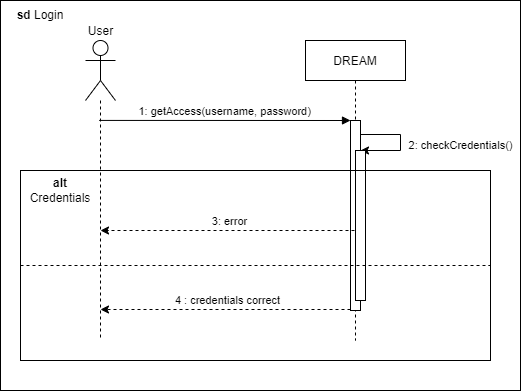
\includegraphics[width=\linewidth]{Images/Use Case/UC1.png}
    \caption{\textit{Platform login} sequence diagram.}
\end{figure}
\newpage

\begin{table}[H]
    \centering
    \begin{tabular}{@{}p{0.25\linewidth}p{0.71\linewidth}@{}}
        \hline
        \textbf{Name} & Interact with another user \\
        \hline
        \textbf{ID} & \usecaseindex{UC.2} ~\\
        \hline
        \textbf{Actors} & TPM, Farmer, Agronomist \\
        \hline
        \textbf{Entry conditions} &
        \begin{itemize}[leftmargin=.4cm,noitemsep,topsep=0pt,before=\vspace{-3mm},after=\vspace{-4mm}]
            \item The platform is running
            \item The user is running the application on his/her device
            \item The user is logged into the system
        \end{itemize} \\
        \hline
        \textbf{Flow of events} &
        \begin{enumerate}[label=\roman*.,leftmargin=.5cm,noitemsep,topsep=0pt,before=\vspace{-3mm},after=\vspace{-4mm}]
            \item The user opens “Chat”
            \item The user clicks on “New Chat”
            \item The user types the username of the other user he/she wants to contact
            \item The user clicks on “Start Conversation”
            \item System creates a new chat between the 2 users
            \item The user types the message he/she wants to send
        \end{enumerate} \\
        \hline
        \textbf{Exit conditions} & The user clicks on “Send”\\
        \hline
        \textbf{Exceptions} &
        \begin{itemize}[leftmargin=.4cm,noitemsep,topsep=0pt,before=\vspace{-3mm},after=\vspace{-4mm}]
            \item If the username of a user or the text of the message is missing, the system does not submit the message and highlights the missing parts.
        \end{itemize} \\
        \hline
    \end{tabular}
    \caption{\textit{Interact with another user} use case description.}
\end{table}
\begin{figure}[H]
    \centering
    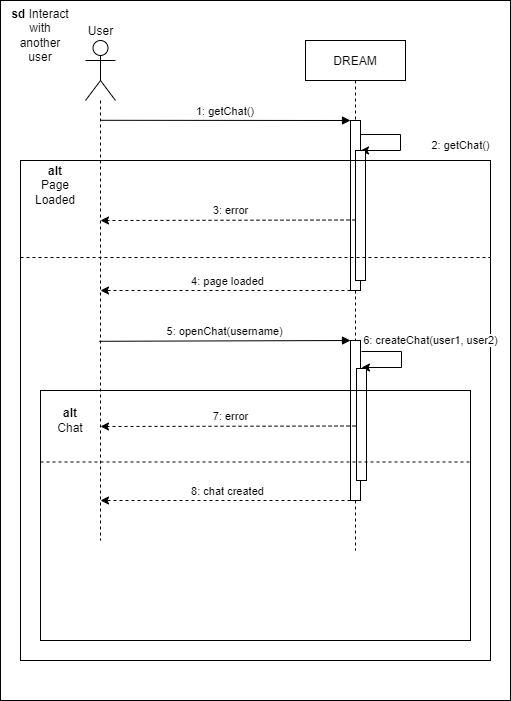
\includegraphics[width=\linewidth]{Images/Use Case/UC2.png}
    \caption{\textit{Interact with another user} sequence diagram.}
\end{figure}
\newpage

\begin{table}[H]
    \centering
    \begin{tabular}{@{}p{0.25\linewidth}p{0.71\linewidth}@{}}
        \hline
        \textbf{Name} & Reply to a new message \\
        \hline
        \textbf{ID} & \usecaseindex{UC.3} ~\\
        \hline
        \textbf{Actors} & TPM, Farmer, Agronomist \\
        \hline
        \textbf{Entry conditions} &
        \begin{itemize}[leftmargin=.4cm,noitemsep,topsep=0pt,before=\vspace{-3mm},after=\vspace{-4mm}]
            \item The platform is running
            \item The user is running the application on his/her device
            \item The user is logged into the system
        \end{itemize} \\
        \hline
        \textbf{Flow of events} &
        \begin{enumerate}[label=\roman*.,leftmargin=.5cm,noitemsep,topsep=0pt,before=\vspace{-3mm},after=\vspace{-4mm}]
            \item The user opens “Chat”
            \item System shows the list of all messages that the user received and highlights the message/s he/she has not read
            \item The user selects the conversation he/she wants to reply
            \item System shows the conversation between the 2 users
            \item The user types the text of the message
        \end{enumerate} \\
        \hline
        \textbf{Exit conditions} & The user clicks on “Send”\\
        \hline
        \textbf{Exceptions} &
        \begin{itemize}[leftmargin=.4cm,noitemsep,topsep=0pt,before=\vspace{-3mm},after=\vspace{-4mm}]
            \item If the text of the message is missing, the system does not submit the message and shows an error message.
        \end{itemize} \\
        \hline
    \end{tabular}
    \caption{\textit{Reply to a new message} use case description.}
\end{table}
\begin{figure}[H]
    \centering
    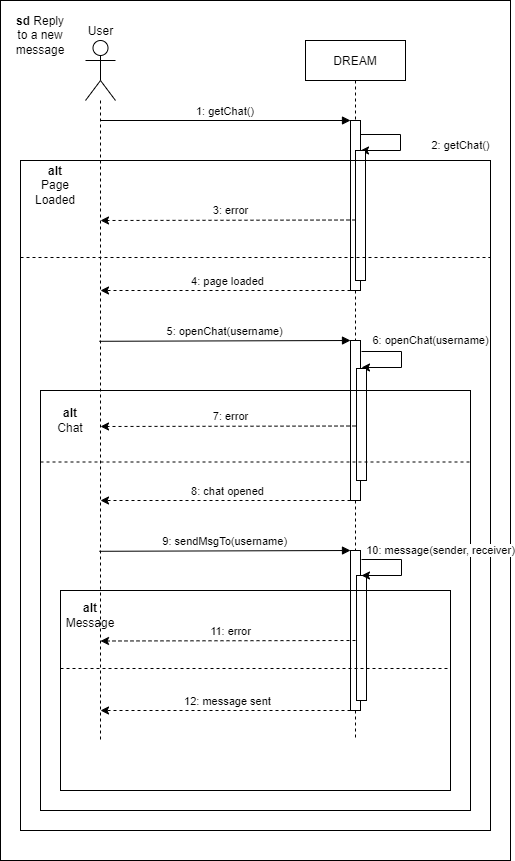
\includegraphics[origin=c,height=1.5\textwidth]{Images/Use Case/UC3.png}
    \caption{\textit{Reply to a new message} sequence diagram.}
\end{figure}
\newpage

\begin{table}[H]
    \centering
    \begin{tabular}{@{}p{0.25\linewidth}p{0.71\linewidth}@{}}
        \hline
        \textbf{Name} & Report of a problem \\
        \hline
        \textbf{ID} & \usecaseindex{UC.4} ~\\
        \hline
        \textbf{Actors} & Farmer \\
        \hline
        \textbf{Entry conditions} &
        \begin{itemize}[leftmargin=.4cm,noitemsep,topsep=0pt,before=\vspace{-3mm},after=\vspace{-4mm}]
            \item The platform is running
            \item The farmer is running the application on his/her device
            \item The farmer is logged into the system
        \end{itemize} \\
        \hline
        \textbf{Flow of events} &
        \begin{enumerate}[label=\roman*.,leftmargin=.5cm,noitemsep,topsep=0pt,before=\vspace{-3mm},after=\vspace{-4mm}]
            \item The farmer goes to “Report a Problem”
            \item The farmer types a title for his/her problem
            \item The farmer inserts the description of the problem faced
            \item The farmer clicks on “Submit”
            \item System retrieves the farmer’s location
            \item System adds the location of the farmer to the form
        \end{enumerate} \\
        \hline
        \textbf{Exit conditions} & The farmer successfully submits the form\\
        \hline
        \textbf{Exceptions} &
        \begin{itemize}[leftmargin=.4cm,noitemsep,topsep=0pt,before=\vspace{-3mm},after=\vspace{-4mm}]
            \item If the form is not submitted, the page is reloaded with all the text inserted by the farmer.
            \item If the form is empty, the system does not submit the data and highlights the missing part.
        \end{itemize} \\
        \hline
    \end{tabular}
    \caption{\textit{Report of a problem} use case description.}
\end{table}
\begin{figure}[H]
    \centering
    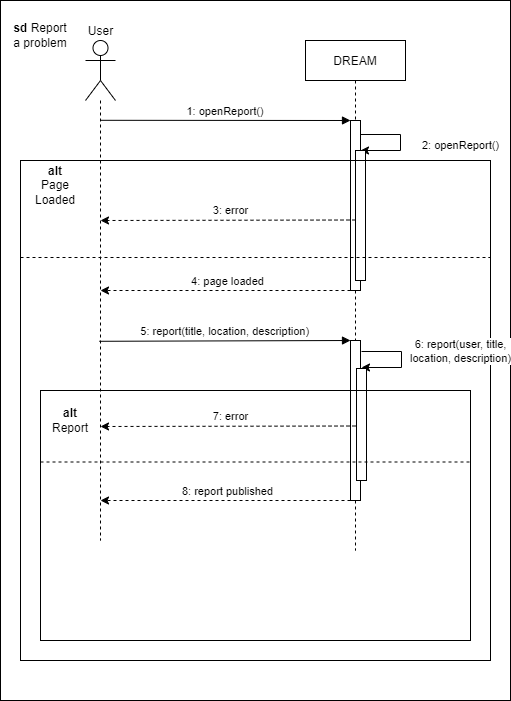
\includegraphics[width=\linewidth]{Images/Use Case/UC4.png}
    \caption{\textit{Report of a problem} sequence diagram.}
\end{figure}
\newpage

\begin{table}[H]
    \centering
    \begin{tabular}{@{}p{0.25\linewidth}p{0.71\linewidth}@{}}
        \hline
        \textbf{Name} & Read about a problem\\
        \hline
        \textbf{ID} & \usecaseindex{UC.5} ~\\
        \hline
        \textbf{Actors} & TPM, Agronomist \\
        \hline
        \textbf{Entry conditions} &
        \begin{itemize}[leftmargin=.4cm,noitemsep,topsep=0pt,before=\vspace{-3mm},after=\vspace{-4mm}]
            \item The platform is running
            \item The user is running the application on his/her device
            \item The user is logged into the system
        \end{itemize} \\
        \hline
        \textbf{Flow of events} &
        \begin{enumerate}[label=\roman*.,leftmargin=.5cm,noitemsep,topsep=0pt,before=\vspace{-3mm},after=\vspace{-4mm}]
            \item The user opens “Report a Problem”
            \item The user selects the area of interest
            \item The user clicks on “Search”
            \item System shows the list of titles of all problems in the area selected
            \item The user selects one in the lists to see the description
            \item System shows the report selected
        \end{enumerate} \\
        \hline
        \textbf{Exit conditions} & System shows the description of the problem selected by the user\\
        \hline
        \textbf{Exceptions} &
        \begin{itemize}[leftmargin=.4cm,noitemsep,topsep=0pt,before=\vspace{-3mm},after=\vspace{-4mm}]
            \item : If in the area there are any report a message is shown: “For the area selected there are no reports”
        \end{itemize} \\
        \hline
    \end{tabular}
    \caption{\textit{Read about a problem} use case description.}
\end{table}
\begin{figure}[H]
    \centering
    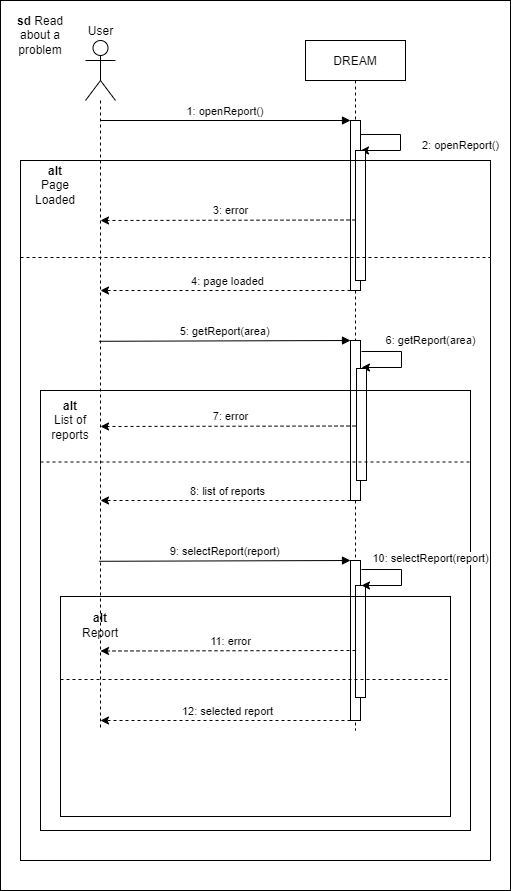
\includegraphics[height=1.5\linewidth]{Images/Use Case/UC5.png}
    \caption{\textit{Read about a problem} sequence diagram.}
\end{figure}
\newpage

\begin{table}[H]
    \centering
    \begin{tabular}{@{}p{0.25\linewidth}p{0.71\linewidth}@{}}
        \hline
        \textbf{Name} & Ask for help\\
        \hline
        \textbf{ID} & \usecaseindex{UC.6} ~\\
        \hline
        \textbf{Actors} & Farmer \\
        \hline
        \textbf{Entry conditions} &
        \begin{itemize}[leftmargin=.4cm,noitemsep,topsep=0pt,before=\vspace{-3mm},after=\vspace{-4mm}]
            \item The platform is running
            \item The farmer is running the application on his/her device
            \item The farmer is logged into the system
        \end{itemize} \\
        \hline
        \textbf{Flow of events} &
        \begin{enumerate}[label=\roman*.,leftmargin=.5cm,noitemsep,topsep=0pt,before=\vspace{-3mm},after=\vspace{-4mm}]
            \item The farmer accesses “Help”
            \item The farmer clicks on “Get support”
            \item The farmer describes how he/she wants to be helped
            \item The farmer clicks on “Submit Request”
            \item The system retrieves the farmer’s location
            \item System adds the location of the farmer to the form
        \end{enumerate} \\
        \hline
        \textbf{Exit conditions} & The farmer successfully submits the form\\
        \hline
        \textbf{Exceptions} &
        \begin{itemize}[leftmargin=.4cm,noitemsep,topsep=0pt,before=\vspace{-3mm},after=\vspace{-4mm}]
            \item If the form is not submitted, the page is reloaded with all the text inserted by the farmer.
            \item If a field of the form is empty, the system does not submit the data and highlights the missing parts.
        \end{itemize} \\
        \hline
    \end{tabular}
    \caption{\textit{Ask for help} use case description.}
\end{table}
\begin{figure}[H]
    \centering
    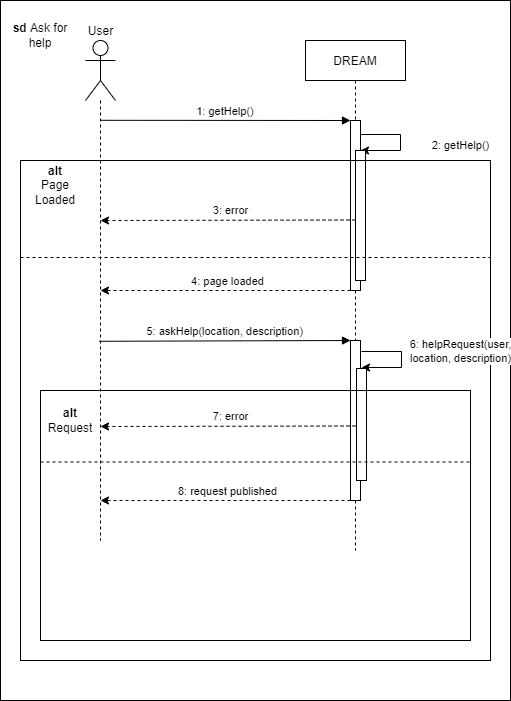
\includegraphics[width=\linewidth]{Images/Use Case/UC6.png}
    \caption{\textit{Ask for help} sequence diagram.}
\end{figure}
\newpage

\begin{table}[H]
    \centering
    \begin{tabular}{@{}p{0.25\linewidth}p{0.71\linewidth}@{}}
        \hline
        \textbf{Name} & Reply to a request of help\\
        \hline
        \textbf{ID} & \usecaseindex{UC.7} ~\\
        \hline
        \textbf{Actors} & Farmer, Agronomist \\
        \hline
        \textbf{Entry conditions} &
        \begin{itemize}[leftmargin=.4cm,noitemsep,topsep=0pt,before=\vspace{-3mm},after=\vspace{-4mm}]
            \item The platform is running
            \item The user is running the application on his/her device
            \item The user is logged into the system
        \end{itemize} \\
        \hline
        \textbf{Flow of events} &
        \begin{enumerate}[label=\roman*.,leftmargin=.5cm,noitemsep,topsep=0pt,before=\vspace{-3mm},after=\vspace{-4mm}]
            \item The user accesses “Help”
            \item System shows the list of all requests of help
            \item The user browses through the requests of help
            \item The user clicks on the request he/she wants to reply
            \item System shows the description of the request
            \item System shows the username and location of the farmer who posted the request
            \item The user types his/her solution to the problem
            \item The user clicks “Reply”
        \end{enumerate} \\
        \hline
        \textbf{Exit conditions} & The user successfully submits his/her reply\\
        \hline
        \textbf{Exceptions} &
        \begin{itemize}[leftmargin=.4cm,noitemsep,topsep=0pt,before=\vspace{-3mm},after=\vspace{-4mm}]
            \item If the reply is not sent, the page and the reply will be reloaded.
            \item If the form is empty, the system does not submit the data and highlights the missing part.
        \end{itemize} \\
        \hline
    \end{tabular}
    \caption{\textit{Reply to a request of help} use case description.}
\end{table}
\begin{figure}[H]
    \centering
    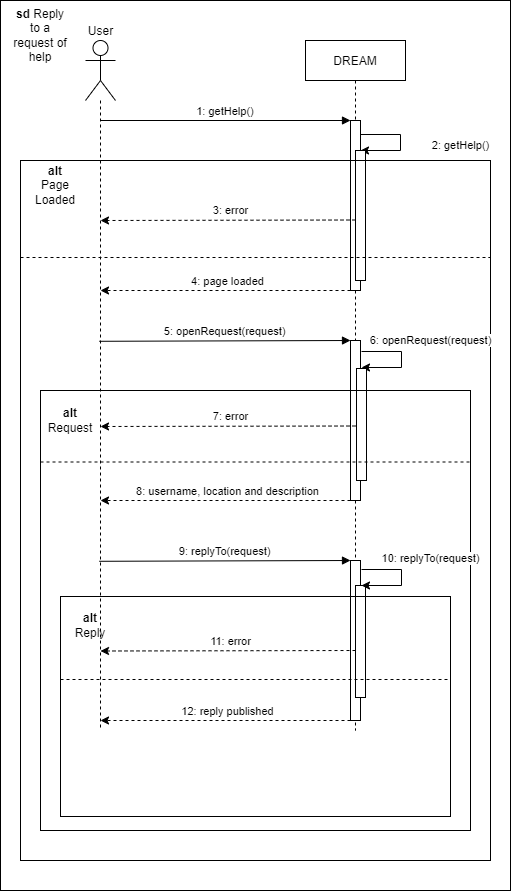
\includegraphics[height=1.5\linewidth]{Images/Use Case/UC7.png}
    \caption{\textit{Reply to a request of help} sequence diagram.}
\end{figure}
\newpage

\begin{table}[H]
    \centering
    \begin{tabular}{@{}p{0.25\linewidth}p{0.71\linewidth}@{}}
        \hline
        \textbf{Name} & Create a new discussion in the Forum\\
        \hline
        \textbf{ID} & \usecaseindex{UC.8} ~\\
        \hline
        \textbf{Actors} & Farmer\\
        \hline
        \textbf{Entry conditions} &
        \begin{itemize}[leftmargin=.4cm,noitemsep,topsep=0pt,before=\vspace{-3mm},after=\vspace{-4mm}]
            \item The platform is running
            \item The farmer is running the application on his/her device
            \item The farmer is logged into the system
        \end{itemize} \\
        \hline
        \textbf{Flow of events} &
        \begin{enumerate}[label=\roman*.,leftmargin=.5cm,noitemsep,topsep=0pt,before=\vspace{-3mm},after=\vspace{-4mm}]
            \item The farmer opens “Forum”
            \item The farmer clicks on “Create new Discussion”
            \item The farmer inserts a title for the discussion
            \item The farmer types the topic of the discussion
            \item The farmer clicks on “Submit Discussion”
            \item System creates the discussion
        \end{enumerate} \\
        \hline
        \textbf{Exit conditions} & The discussion is successfully submitted and the system updates “Forum”\\
        \hline
        \textbf{Exceptions} &
        \begin{itemize}[leftmargin=.4cm,noitemsep,topsep=0pt,before=\vspace{-3mm},after=\vspace{-4mm}]
            \item If the discussion is not submitted, the page and the form is reloaded.
            \item If a field of the form is empty, the system does not submit the data and highlights the missing parts.
        \end{itemize} \\
        \hline
    \end{tabular}
    \caption{\textit{Create a new discussion in the Forum} use case description.}
\end{table}
\begin{figure}[H]
    \centering
    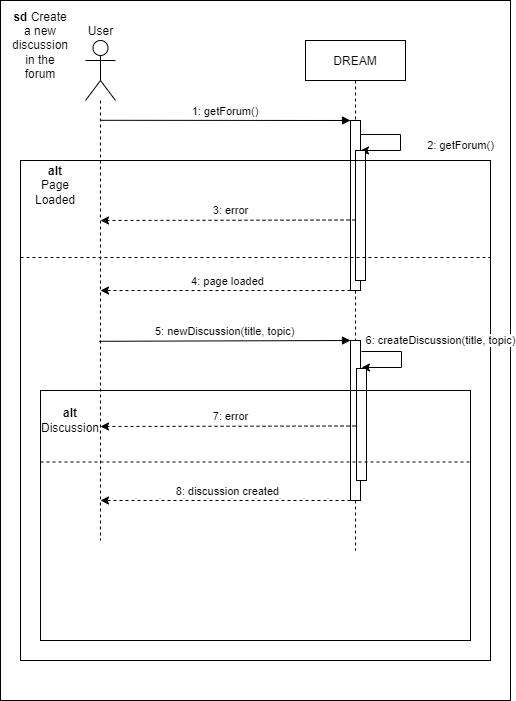
\includegraphics[width=\linewidth]{Images/Use Case/UC8.png}
    \caption{\textit{Create a new discussion in the Forum} sequence diagram.}
\end{figure}
\newpage

\begin{table}[H]
    \centering
    \begin{tabular}{@{}p{0.25\linewidth}p{0.71\linewidth}@{}}
        \hline
        \textbf{Name} & Reply to a discussion in the Forum\\
        \hline
        \textbf{ID} & \usecaseindex{UC.9} ~\\
        \hline
        \textbf{Actors} & Farmer\\
        \hline
        \textbf{Entry conditions} &
        \begin{itemize}[leftmargin=.4cm,noitemsep,topsep=0pt,before=\vspace{-3mm},after=\vspace{-4mm}]
            \item The platform is running
            \item The farmer is running the application on his/her device
            \item The farmer is logged into the system
        \end{itemize} \\
        \hline
        \textbf{Flow of events} &
        \begin{enumerate}[label=\roman*.,leftmargin=.5cm,noitemsep,topsep=0pt,before=\vspace{-3mm},after=\vspace{-4mm}]
            \item The farmer opens “Forum”
            \item System shows the list of all discussions in the forum
            \item The farmer browses through the discussions already created
            \item The farmer selects the topic he/she wants to reply
            \item System shows the replies to the topic
            \item The farmer types his/her reply
            \item The farmer clicks on “Send”
        \end{enumerate} \\
        \hline
        \textbf{Exit conditions} & The reply to the topic is successfully submitted\\
        \hline
        \textbf{Exceptions} &
        \begin{itemize}[leftmargin=.4cm,noitemsep,topsep=0pt,before=\vspace{-3mm},after=\vspace{-4mm}]
            \item If reply is not submitted, the discussion and the reply are reloaded.
            \item If a field of the form is empty, the system does not submit the data and highlights the reply area.
        \end{itemize} \\
        \hline
    \end{tabular}
    \caption{\textit{Reply to a discussion in the Forum} use case description.}
\end{table}
\begin{figure}[H]
    \centering
    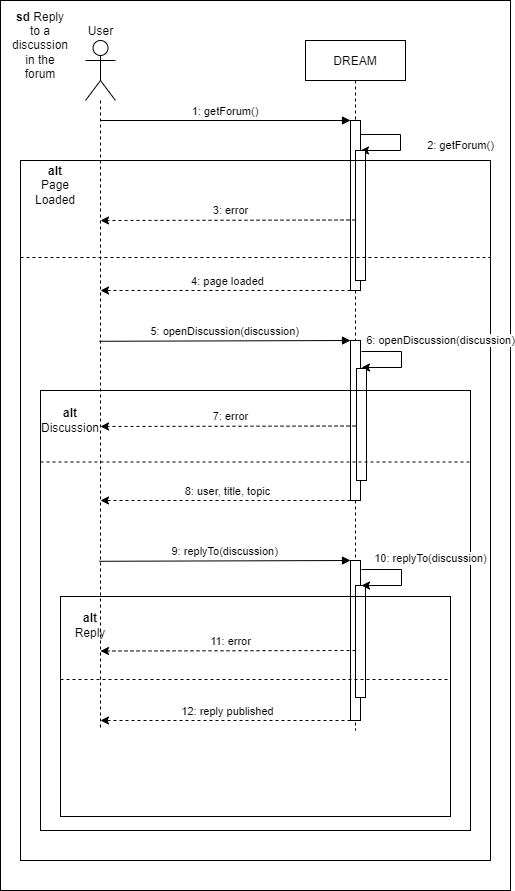
\includegraphics[height=1.5\linewidth]{Images/Use Case/UC9.png}
    \caption{\textit{Reply to a discussion in the Forum} sequence diagram.}
\end{figure}
\newpage

\begin{table}[H]
    \centering
    \begin{tabular}{@{}p{0.25\linewidth}p{0.71\linewidth}@{}}
        \hline
        \textbf{Name} & Get suggestions\\
        \hline
        \textbf{ID} & \usecaseindex{UC.10} ~\\
        \hline
        \textbf{Actors} & Agronomist, Farmer\\
        \hline
        \textbf{Entry conditions} &
        \begin{itemize}[leftmargin=.4cm,noitemsep,topsep=0pt,before=\vspace{-3mm},after=\vspace{-4mm}]
            \item The platform is running
            \item The user is running the application on his/her device
            \item The user is logged into the system
        \end{itemize} \\
        \hline
        \textbf{Flow of events} &
        \begin{enumerate}[label=\roman*.,leftmargin=.5cm,noitemsep,topsep=0pt,before=\vspace{-3mm},after=\vspace{-4mm}]
            \item The user opens “WikiFarm”
            \item The user selects the zone
            \item The user inserts the type of production
            \item The user clicks on “Get Suggestions”
            \item System shows a list of all the compatible fertilizer, regarding the data inserted
            \item System shows a list of all the compatible crops, regarding the data inserted
        \end{enumerate} \\
        \hline
        \textbf{Exit conditions} & The user closes DREAM or the user opens another section\\
        \hline
        \textbf{Exceptions} &
        \begin{itemize}[leftmargin=.4cm,noitemsep,topsep=0pt,before=\vspace{-3mm},after=\vspace{-4mm}]
            \item If for the request there is no solution, an error message is displayed, and the farmer is brought to the section of suggestions.
            \item If a field of the form is empty, the system does not submit the data and highlights the missing parts.
        \end{itemize} \\
        \hline
    \end{tabular}
    \caption{\textit{Get suggestions} use case description.}
\end{table}
\begin{figure}[H]
    \centering
    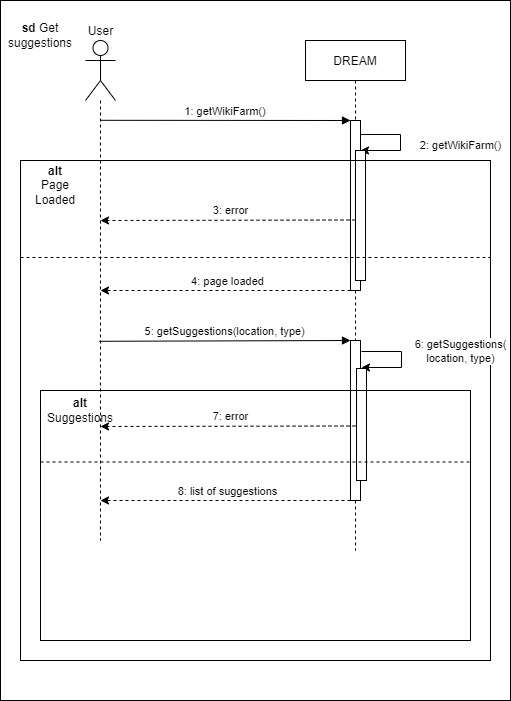
\includegraphics[width=\linewidth]{Images/Use Case/UC10.png}
    \caption{\textit{Get suggestions} sequence diagram.}
\end{figure}
\newpage

\begin{table}[H]
    \centering
    \begin{tabular}{@{}p{0.25\linewidth}p{0.71\linewidth}@{}}
        \hline
        \textbf{Name} & Insert data of production\\
        \hline
        \textbf{ID} & \usecaseindex{UC.11} ~\\
        \hline
        \textbf{Actors} & Farmer\\
        \hline
        \textbf{Entry conditions} &
        \begin{itemize}[leftmargin=.4cm,noitemsep,topsep=0pt,before=\vspace{-3mm},after=\vspace{-4mm}]
            \item The platform is running
            \item The farmer is running the application on his/her device
            \item The farmer is logged into the system
        \end{itemize} \\
        \hline
        \textbf{Flow of events} &
        \begin{enumerate}[label=\roman*.,leftmargin=.5cm,noitemsep,topsep=0pt,before=\vspace{-3mm},after=\vspace{-4mm}]
            \item The farmer opens “Report Production”
            \item The farmer types the type of production
            \item The farmer types the crop planted
            \item The farmer inserts the amount produced
            \item The farmer inserts the amount of land dedicated to the production
            \item The farmer clicks on “Finish”
            \item Using the sensors in the distribution system, DREAM retrieves the amount of water used by farmer
            \item Using the sensors in the land, DREAM retrieves the humidity of the soil
            \item System retrieves the farmer’s location
        \end{enumerate} \\
        \hline
        \textbf{Exit conditions} & System combines data inserted by the farmer with the ones retrieved and it stores them into the database with the correct date.\\
        \hline
        \textbf{Exceptions} &
        \begin{itemize}[leftmargin=.4cm,noitemsep,topsep=0pt,before=\vspace{-3mm},after=\vspace{-4mm}]
            \item If a field of the form is empty, the system does not submit the data and highlights the missing parts.
            \item If the farmer clicks on “Next”, the system stores the data typed and loads a new page to insert another production report.
        \end{itemize} \\
        \hline
    \end{tabular}
    \caption{\textit{Insert data of production} use case description.}
\end{table}
\begin{figure}[H]
    \centering
    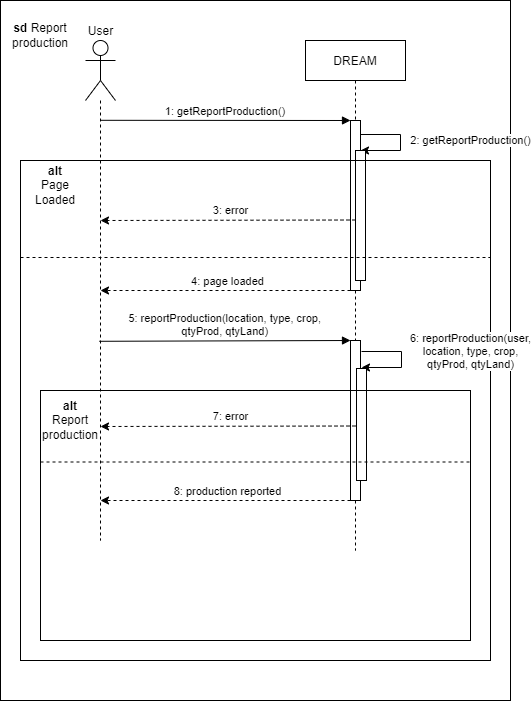
\includegraphics[width=\linewidth]{Images/Use Case/UC11.png}
    \caption{\textit{Insert data of production} sequence diagram.}
\end{figure}
\newpage

\begin{table}[H]
    \centering
    \begin{tabular}{@{}p{0.25\linewidth}p{0.71\linewidth}@{}}
        \hline
        \textbf{Name} & Search data of production\\
        \hline
        \textbf{ID} & \usecaseindex{UC.12} ~\\
        \hline
        \textbf{Actors} & TPM, Agronomist\\
        \hline
        \textbf{Entry conditions} &
        \begin{itemize}[leftmargin=.4cm,noitemsep,topsep=0pt,before=\vspace{-3mm},after=\vspace{-4mm}]
            \item The platform is running
            \item The user is running the application on his/her device
            \item The user is logged into the system
        \end{itemize} \\
        \hline
        \textbf{Flow of events} &
        \begin{enumerate}[label=\roman*.,leftmargin=.5cm,noitemsep,topsep=0pt,before=\vspace{-3mm},after=\vspace{-4mm}]
            \item The user opens “Report Production”
            \item The user types the username of the farmer he/she wants to visualize
            \item System shows search in the database all the data inserted by the farmer
            \item System shows search in the database all the data inserted by the farmer
        \end{enumerate} \\
        \hline
        \textbf{Exit conditions} & The user closes DREAM or opens another section of the system.\\
        \hline
        \textbf{Exceptions} &
        \begin{itemize}[leftmargin=.4cm,noitemsep,topsep=0pt,before=\vspace{-3mm},after=\vspace{-4mm}]
            \item If the farmer selected has not already reported data of production, the system shows a message: “The farmer selected has no data of production inserted”
        \end{itemize} \\
        \hline
    \end{tabular}
    \caption{\textit{ISearch data of production} use case description.}
\end{table}
\begin{figure}[H]
    \centering
    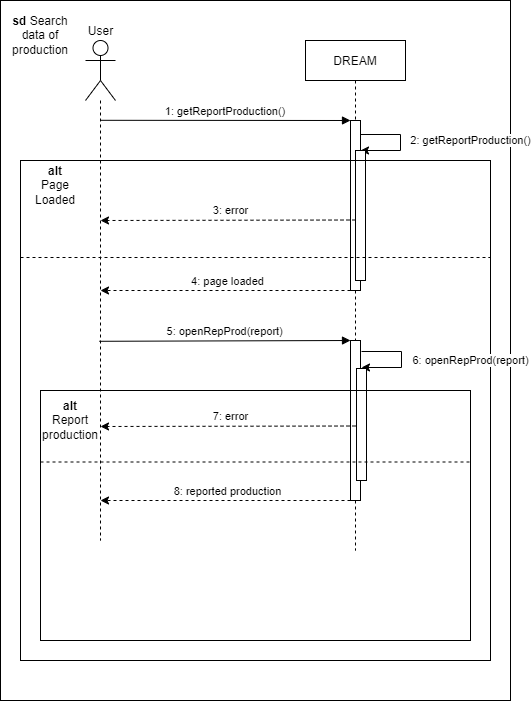
\includegraphics[width=\linewidth]{Images/Use Case/UC12.png}
    \caption{\textit{Search data of production} sequence diagram.}
\end{figure}
\newpage

\begin{table}[H]
    \centering
    \begin{tabular}{@{}p{0.25\linewidth}p{0.71\linewidth}@{}}
        \hline
        \textbf{Name} & Generation of the ranking of the farmers\\
        \hline
        \textbf{ID} & \usecaseindex{UC.13} ~\\
        \hline
        \textbf{Actors} &TPM, Agronomist\\
        \hline
        \textbf{Entry conditions} &
        \begin{itemize}[leftmargin=.4cm,noitemsep,topsep=0pt,before=\vspace{-3mm},after=\vspace{-4mm}]
            \item The platform is running
            \item The user is running the application on the user’s device
            \item The user is logged into the system
        \end{itemize} \\
        \hline
        \textbf{Flow of events} &
        \begin{enumerate}[label=\roman*.,leftmargin=.5cm,noitemsep,topsep=0pt,before=\vspace{-3mm},after=\vspace{-4mm}]
            \item The user opens “Ranking”
            \item The user selects the zone of interest
            \item The user clicks “Search”
            \item System computes the evaluation of the performance of all the farmers in the selected area
            \item System shows the list of all farmers from the best performing to the worst
        \end{enumerate} \\
        \hline
        \textbf{Exit conditions} & The user closes DREAM or opens another section of the system\\
        \hline
        \textbf{Exceptions} &
        \begin{itemize}[leftmargin=.4cm,noitemsep,topsep=0pt,before=\vspace{-3mm},after=\vspace{-4mm}]
            \item In case of ties, farmers are ordered alphabetically.
            \item If no area is selected, the ranking will be based on all the farmers in Telangana.
        \end{itemize} \\
        \hline
    \end{tabular}
    \caption{\textit{Generation of the ranking of the farmers} use case description.}
\end{table}
\begin{figure}[H]
    \centering
    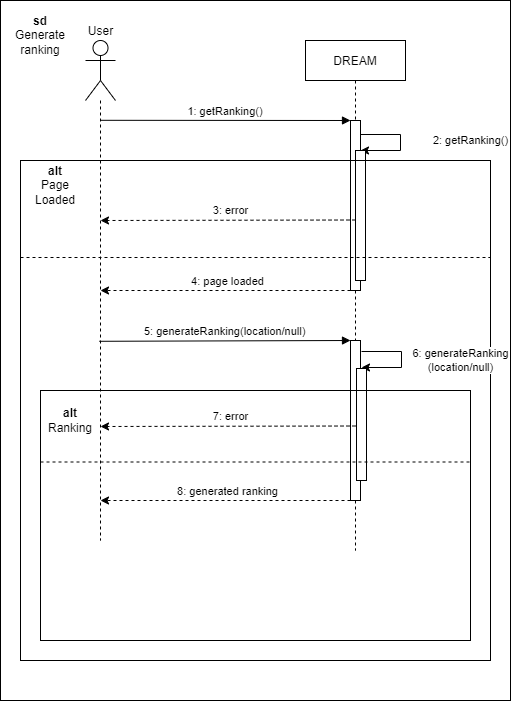
\includegraphics[width=\linewidth]{Images/Use Case/UC13.png}
    \caption{\textit{Generation of the ranking of the farmers} sequence diagram.}
\end{figure}
\newpage

\begin{table}[H]
    \centering
    \begin{tabular}{@{}p{0.25\linewidth}p{0.71\linewidth}@{}}
        \hline
        \textbf{Name} & Checking the weather forecast\\
        \hline
        \textbf{ID} & \usecaseindex{UC.14} ~\\
        \hline
        \textbf{Actors} & Farmer, Agronomist\\
        \hline
        \textbf{Entry conditions} &
        \begin{itemize}[leftmargin=.4cm,noitemsep,topsep=0pt,before=\vspace{-3mm},after=\vspace{-4mm}]
            \item The platform is running
            \item The user is running the application on the user’s device
            \item The user is logged into the system
        \end{itemize} \\
        \hline
        \textbf{Flow of events} &
        \begin{enumerate}[label=\roman*.,leftmargin=.5cm,noitemsep,topsep=0pt,before=\vspace{-3mm},after=\vspace{-4mm}]
            \item The user opens “Weather”
            \item The user selects the zone of interest
            \item The user selects the temporal slot for the forecast
            \item The user clicks “Search”
            \item System accesses the Telangana’s weather portal
            \item System requests forecast for the time slot and zone chosen by the user
            \item System shows the weather forecast chosen
        \end{enumerate} \\
        \hline
        \textbf{Exit conditions} & The user closes the page or decides to do another operation.\\
        \hline
        \textbf{Exceptions} &
        \begin{itemize}[leftmargin=.4cm,noitemsep,topsep=0pt,before=\vspace{-3mm},after=\vspace{-4mm}]
            \item In case of service disruption caused by bad weather, the system shows an error message, and the user is brought to the home page of the system.
            \item If the time slot is greater than 7 days, the system shows the average forecast for the area and period selected.
        \end{itemize} \\
        \hline
    \end{tabular}
    \caption{\textit{Checking the weather forecast} use case description.}
\end{table}
\begin{figure}[H]
    \centering
    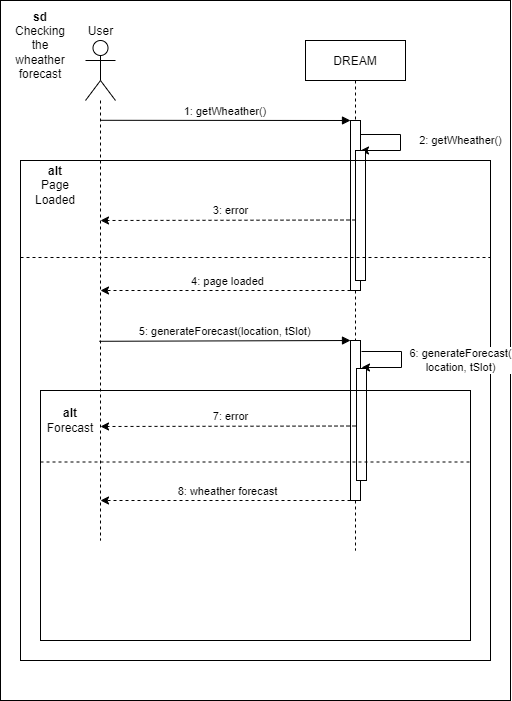
\includegraphics[width=\linewidth]{Images/Use Case/UC14.png}
    \caption{\textit{Checking the weather forecast} sequence diagram.}
\end{figure}
\newpage

\begin{table}[H]
    \centering
    \begin{tabular}{@{}p{0.25\linewidth}p{0.71\linewidth}@{}}
        \hline
        \textbf{Name} & Checking the schedule\\
        \hline
        \textbf{ID} & \usecaseindex{UC.15} ~\\
        \hline
        \textbf{Actors} & Agronomist\\
        \hline
        \textbf{Entry conditions} &
        \begin{itemize}[leftmargin=.4cm,noitemsep,topsep=0pt,before=\vspace{-3mm},after=\vspace{-4mm}]
            \item The platform is running
            \item The Agronomist is running the application
            \item The Agronomist is logged into the system
        \end{itemize} \\
        \hline
        \textbf{Flow of events} &
        \begin{enumerate}[label=\roman*.,leftmargin=.5cm,noitemsep,topsep=0pt,before=\vspace{-3mm},after=\vspace{-4mm}]
            \item The agronomist opens “Agenda”
            \item The agronomist selects the day of interest
            \item The agronomist clicks “Search”
            \item System shows the list of all the events planned for that day
            \item The agronomist selects the event he/she wants to visualize
            \item System shows the details for the event selected
        \end{enumerate} \\
        \hline
        \textbf{Exit conditions} & The agronomist closes the page or decides to do another operation.\\
        \hline
        \textbf{Exceptions} &
        \begin{itemize}[leftmargin=.4cm,noitemsep,topsep=0pt,before=\vspace{-3mm},after=\vspace{-4mm}]
            \item If in the date selected there are no events planned, the system will show a blank page with the text “No events for the date selected”.
        \end{itemize} \\
        \hline
    \end{tabular}
    \caption{\textit{Checking the schedule} use case description.}
\end{table}
\begin{figure}[H]
    \centering
    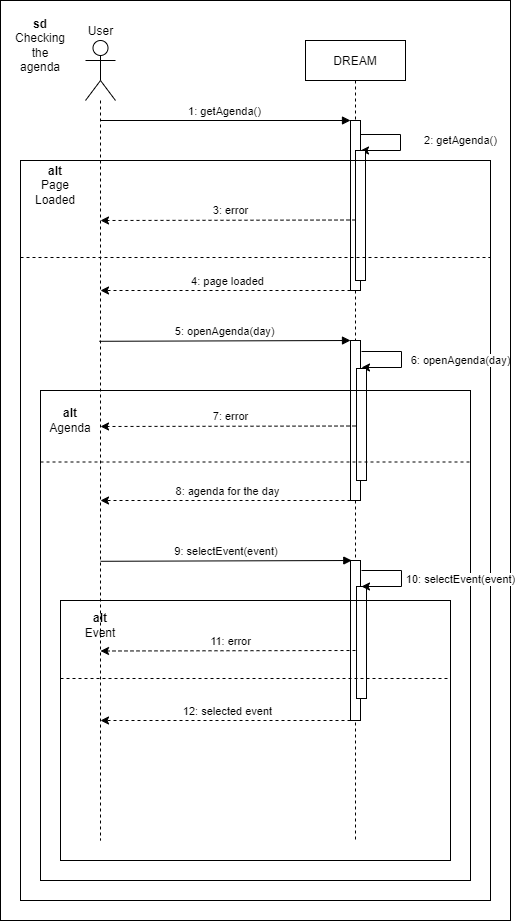
\includegraphics[height=1.5\linewidth]{Images/Use Case/UC15.png}
    \caption{\textit{Checking the schedule} sequence diagram.}
\end{figure}
\newpage

\begin{table}[H]
    \centering
    \begin{tabular}{@{}p{0.25\linewidth}p{0.71\linewidth}@{}}
        \hline
        \textbf{Name} & Reporting a visit to a farmer\\
        \hline
        \textbf{ID} & \usecaseindex{UC.16} ~\\
        \hline
        \textbf{Actors} & Agronomist\\
        \hline
        \textbf{Entry conditions} &
        \begin{itemize}[leftmargin=.4cm,noitemsep,topsep=0pt,before=\vspace{-3mm},after=\vspace{-4mm}]
            \item The platform is running
            \item The Agronomist is running the application
            \item The Agronomist is logged into the system
        \end{itemize} \\
        \hline
        \textbf{Flow of events} &
        \begin{enumerate}[label=\roman*.,leftmargin=.5cm,noitemsep,topsep=0pt,before=\vspace{-3mm},after=\vspace{-4mm}]
            \item The agronomist opens “Agenda”
            \item The agronomist selects the current day
            \item The agronomist clicks “Search”
            \item System shows the list of all the events planned for that day
            \item The agronomist selects the event he/she has just concluded
            \item System shows the details of the event selected
            \item The agronomist clicks “Upload Report”
            \item The agronomist types the report of the visit
            \item The agronomist clicks “Visit concluded”
        \end{enumerate} \\
        \hline
        \textbf{Exit conditions} & The report of the visit is successfully stored in the system.\\
        \hline
        \textbf{Exceptions} &
        \begin{itemize}[leftmargin=.4cm,noitemsep,topsep=0pt,before=\vspace{-3mm},after=\vspace{-4mm}]
            \item If the upload of the report fails an error message is shown and the agronomist is asked to repeat the operation.
        \end{itemize} \\
        \hline
    \end{tabular}
    \caption{\textit{Reporting a visit to a farmer} use case description.}
\end{table}
\begin{figure}[H]
    \centering
    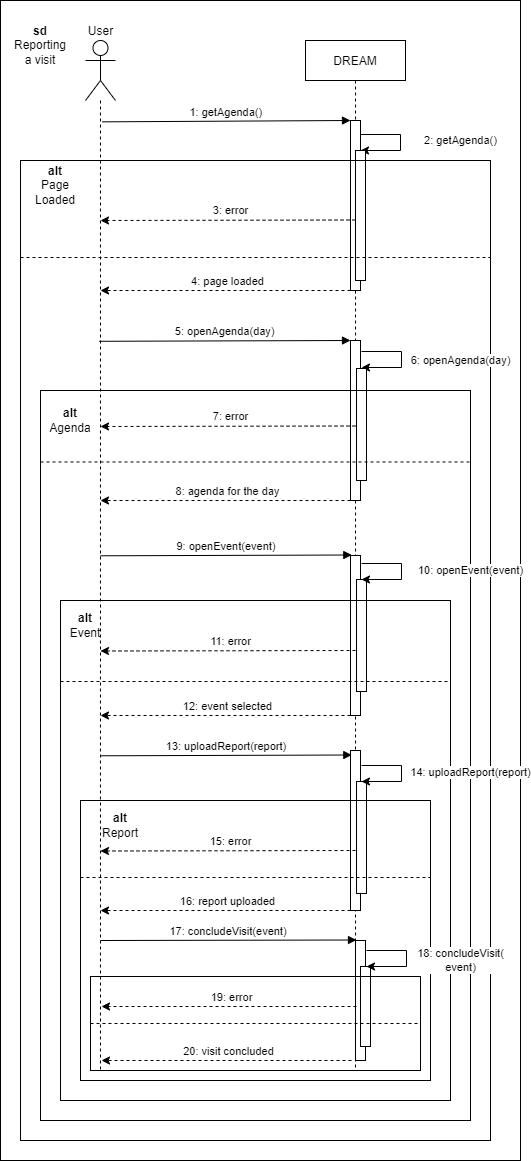
\includegraphics[height=1.5\linewidth]{Images/Use Case/UC16.png}
    \caption{\textit{Reporting a visit to a farmer} sequence diagram.}
\end{figure}
\newpage

\begin{table}[H]
    \centering
    \begin{tabular}{@{}p{0.25\linewidth}p{0.71\linewidth}@{}}
        \hline
        \textbf{Name} & Changing the schedule\\
        \hline
        \textbf{ID} & \usecaseindex{UC.17} ~\\
        \hline
        \textbf{Actors} & Agronomist\\
        \hline
        \textbf{Entry conditions} &
        \begin{itemize}[leftmargin=.4cm,noitemsep,topsep=0pt,before=\vspace{-3mm},after=\vspace{-4mm}]
            \item The platform is running
            \item The Agronomist is running the application
            \item The Agronomist is logged into the system
        \end{itemize} \\
        \hline
        \textbf{Flow of events} &
        \begin{enumerate}[label=\roman*.,leftmargin=.5cm,noitemsep,topsep=0pt,before=\vspace{-3mm},after=\vspace{-4mm}]
            \item The agronomist opens “Agenda”
            \item The agronomist selects the day
            \item The agronomist clicks “Search”
            \item System shows the list of all the events planned for that day
            \item The agronomist selects the event he/she has not done
            \item The agronomist clicks “Change Date”
            \item The agronomist selects the new date for the visit
            \item The agronomist selects the new time for the visit
            \item The agronomist clicks “Upload changes”
        \end{enumerate} \\
        \hline
        \textbf{Exit conditions} & The system successfully updates the agronomist’s “Agenda”\\
        \hline
        \textbf{Exceptions} &
        \begin{itemize}[leftmargin=.4cm,noitemsep,topsep=0pt,before=\vspace{-3mm},after=\vspace{-4mm}]
            \item If the visit is overlapping with another event, a message is displayed: “There is another event for that time and date, please choose another slot.” The system brings the agronomist to the page where he/she could modify the new date and time.
        \end{itemize} \\
        \hline
    \end{tabular}
    \caption{\textit{Changing the schedule} use case description.}
\end{table}
\begin{figure}[H]
    \centering
    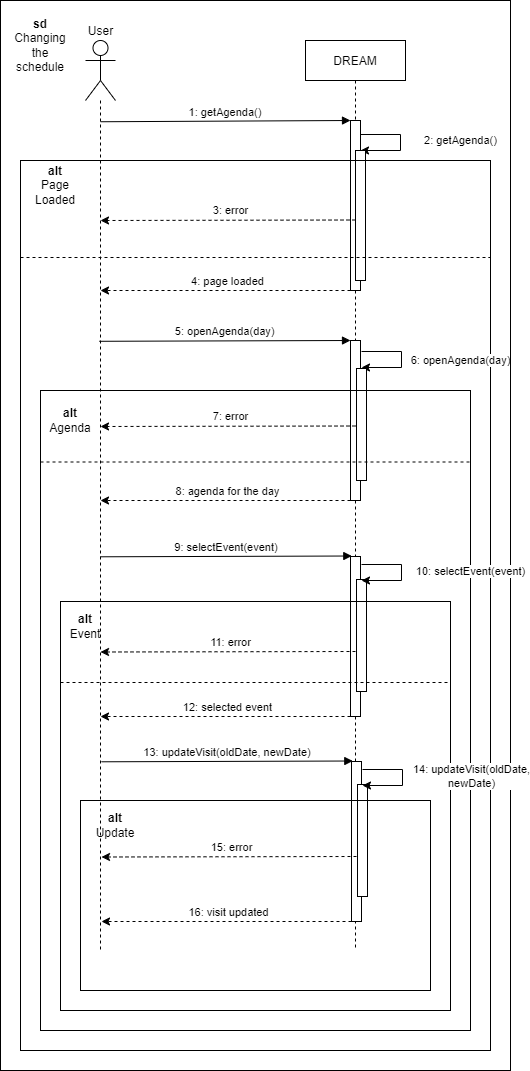
\includegraphics[height=1.5\linewidth]{Images/Use Case/UC17.png}
    \caption{\textit{Changing the schedule} sequence diagram.}
\end{figure}
\newpage

\begin{table}[H]
    \centering
    \begin{tabular}{@{}p{0.25\linewidth}p{0.71\linewidth}@{}}
        \hline
        \textbf{Name} & Creating a new event in the schedule\\
        \hline
        \textbf{ID} & \usecaseindex{UC.18} ~\\
        \hline
        \textbf{Actors} & Agronomist\\
        \hline
        \textbf{Entry conditions} &
        \begin{itemize}[leftmargin=.4cm,noitemsep,topsep=0pt,before=\vspace{-3mm},after=\vspace{-4mm}]
            \item The platform is running
            \item The Agronomist is running the application
            \item The Agronomist is logged into the system
        \end{itemize} \\
        \hline
        \textbf{Flow of events} &
        \begin{enumerate}[label=\roman*.,leftmargin=.5cm,noitemsep,topsep=0pt,before=\vspace{-3mm},after=\vspace{-4mm}]
            \item The agronomist opens “Agenda”
            \item The agronomist selects a day
            \item The agronomist clicks “Search”
            \item System shows the list of all the events planned for that day
            \item The agronomist clicks “New Event”
            \item The agronomist inserts a title for the event
            \item The agronomist selects the time for the visit
            \item The agronomist inserts the username of the farmer he/she has to visit
            \item The agronomist clicks “Create event”
            \item System retrieves the location of the farmer
            \item System adds the location to the event
        \end{enumerate} \\
        \hline
        \textbf{Exit conditions} & System successfully creates the event and successfully updates the agronomist’s “Agenda”\\
        \hline
        \textbf{Exceptions} &
        \begin{itemize}[leftmargin=.4cm,noitemsep,topsep=0pt,before=\vspace{-3mm},after=\vspace{-4mm}]
            \item If the visit is overlapping with another event, a message is displayed: “There is another event for that time and date, please choose another slot.” The system brings the agronomist to the page where he/she could modify the new date and time.
        \end{itemize} \\
        \hline
    \end{tabular}
    \caption{\textit{Creating a new event in the schedule} use case description.}
\end{table}
\begin{figure}[H]
    \centering
    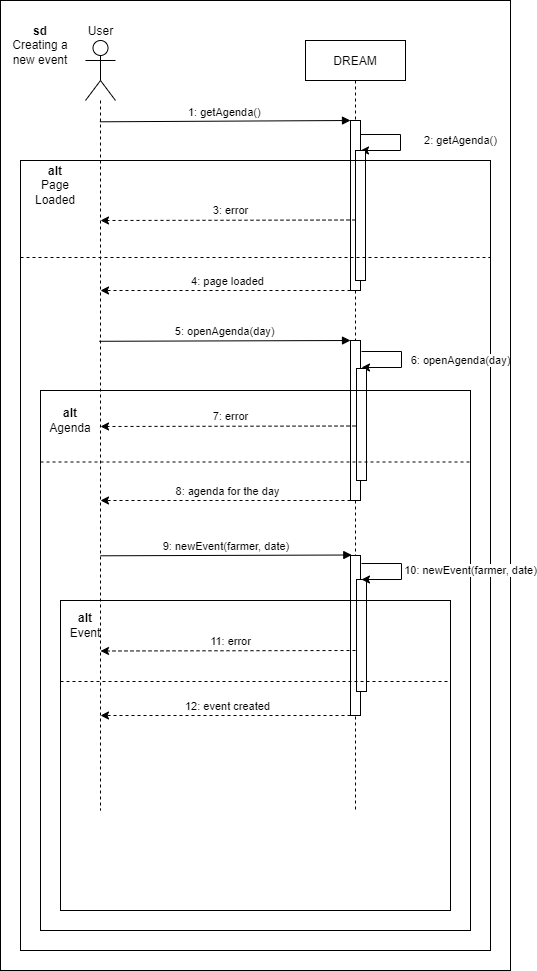
\includegraphics[height=1.5\linewidth]{Images/Use Case/UC18.png}
    \caption{\textit{Creating a new event in the schedule} sequence diagram.}
\end{figure}
\newpage

\begin{table}[H]
    \centering
    \begin{tabular}{@{}p{0.25\linewidth}p{0.71\linewidth}@{}}
        \hline
        \textbf{Name} & Visualize the report of an agronomist’s visit\\
        \hline
        \textbf{ID} & \usecaseindex{UC.19} ~\\
        \hline
        \textbf{Actors} & TPM\\
        \hline
        \textbf{Entry conditions} &
        \begin{itemize}[leftmargin=.4cm,noitemsep,topsep=0pt,before=\vspace{-3mm},after=\vspace{-4mm}]
            \item The platform is running
            \item The TPM is running the application
            \item The TPM is logged into the system
        \end{itemize} \\
        \hline
        \textbf{Flow of events} &
        \begin{enumerate}[label=\roman*.,leftmargin=.5cm,noitemsep,topsep=0pt,before=\vspace{-3mm},after=\vspace{-4mm}]
            \item The TPM opens “Visualize Initiatives”
            \item The TPM types the username of the farmer
            \item he TPM clicks “Search”
            \item System shows a list with all the reports associated with the farmer selected
            \item The TPM selects the report he/she wants to visualize
            \item System shows the selected report
        \end{enumerate} \\
        \hline
        \textbf{Exit conditions} & The TPM closes DREAM or selects another operation.\\
        \hline
        \textbf{Exceptions} &
        \begin{itemize}[leftmargin=.4cm,noitemsep,topsep=0pt,before=\vspace{-3mm},after=\vspace{-4mm}]
            \item If the farmer selected has not yet associated with a report, the system shows a message:” The farmer selected has no reports”.
        \end{itemize} \\
        \hline
    \end{tabular}
    \caption{\textit{Visualize the report of an agronomist’s visit} use case description.}
\end{table}
\begin{figure}[H]
    \centering
    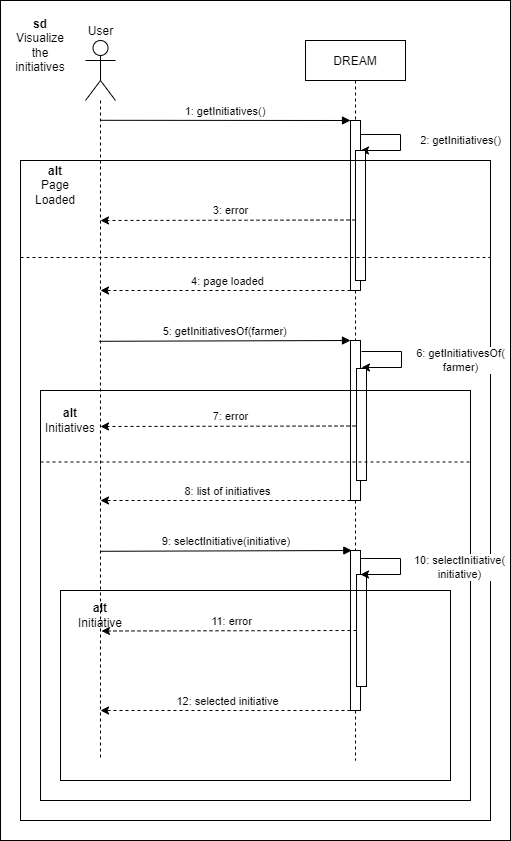
\includegraphics[height=1.5\linewidth]{Images/Use Case/UC19.png}
    \caption{\textit{Visualize the report of an agronomist’s visit} sequence diagram.}
\end{figure}
\newpage

\subsection{Functional Requirements}
In this section, it is given a complete description of the functional requirements of the system.
\subsubsection{Requirements}
\begin{enumerate} [label=\textbf{R.\arabic*}]
    \item Data in the system are never deleted 
    \item System shall retrieve the data from a sensor of humidity in a land
    \item System shall update data of humidity in land every hour
    \item System shall retrieve the amount of water supplied to a farmer
    \item System shall weekly update the amount of water consumed by a farmers 
    \item System shall compute a ranking of the farmers’ performances
    \item System shall allow any user to communicate with any other user using the chat function
    \item System shall allow a farmer to insert his/her type of production
    \item System shall store the location of each farmer
    \item System shall store all the types of production of each farmer
    \item System shall allow a farmer to filter the type of data he/she wants to visualize
    \item System shall receive information about local weather forecast
    \item System shall allow a farmer to visualize the weather forecast
    \item System shall store all the fertilizers available in Telangana
    \item System shall suggest fertilizers based on the retrieved data
    \item System shall store all crops that can be planted in Telangana
    \item System shall suggest crops based on the retrieved data
    \item System shall allow a farmer to insert his/her data of production
    \item System shall store all data of production of farmers
    \item System shall allow a farmer to insert data about a problem that he/she faced 
    \item System shall store all data of problems faced by farmers
    \item System shall allow a resilient farmer to share best practices with other farmers
    \item System shall allow a farmer to ask for help
    \item System shall allow a farmer to reply to a request of help
    \item System shall allow a farmer to create a new discussion in the Forum
    \item System shall allow a farmer to reply to a discussion in the Forum
    \item System shall allow an agronomist to select the area he/she is responsible of
    \item System shall allow an agronomist to visualize a request of help in the area he/she is responsible of
    \item System shall allow an agronomist to reply to a request of help in the area he/she is responsible of
    \item System shall allow an agronomist to visualize the weather forecast for the area he/she is responsible of
    \item System shall allow an agronomist to visualize the performances of farmers in the area he/she is responsible of
    \item System shall allow an agronomist to visualize data of production inserted by farmers
    \item System shall allow an agronomist to visualize problems reported by farmers in the area he/she is responsible of
    \item System shall store the daily plan of all agronomists
    \item System shall allow an agronomist to visualize his/her daily plan
    \item System shall allow an agronomist to update his/her daily plan
    \item System shall allow an agronomist to confirm his/her daily plan
    \item System shall allow an agronomist to insert the deviations from his/her original daily plan
    \item System shall store all the initiatives took by a farmer and an agronomist
    \item System shall allow an agronomist to insert an initiative he/she proposed to a farmer
    \item System shall allow TPM to visualize the ranking of farmers’ performances
    \item System shall allow TPM to visualize data about the production of a farmer
    \item System shall allow TPM to visualize the problems reported by farmers
    \item System shall allow TPM to visualize initiatives taken by agronomist during his/her visits
    \item System shall allow TPM to ask to a resilient farmer to share best practices
    \item System shall allow TPM to signal bad farmers to Agronomists
    \item System shall allow any user to access through a browser
    \item System shall allow any user to log in using his/her credentials
    \item System shall give access to any user who have the right permission. For example, a farmer could not access to “Agenda”
\end{enumerate}

\subsubsection{Mapping Goals on Requirements and Domain Assumptions}
\begin{enumerate}[label=\textbf{G.\arabic*}]
    \item Make available/Share the weather forecasts collected by Telangana
    \begin{itemize} [label =]
        \item R1 - Data in the system are never deleted
        \item R11 - System shall allow a farmer to filter the type of data he/she wants to visualize
        \item R12 - System shall receive information about local weather forecast
        \item R13 - System shall allow a farmer to visualize the weather forecast
        \item R30 - System shall allow an agronomist to visualize the weather forecast for the area he/she is responsible of
        \item DA1 - All Telangana’s people, who interact with system, have an internet connection
        \item DA2 - All Telangana’s people, who interact with system, have access to a browser
        \item DA18 - Weather forecast for a specific zone is always available
    \end{itemize}
    \item Create an anticipatory model for Telangana’s food system
    \begin{itemize} [label =]
        \item R1 - Data in the system are never deleted
        \item R2 - System shall retrieve the data from a sensor of humidity in a land
        \item R3 - System shall update data of humidity in land every hour
        \item R4 - System shall retrieve the amount of water supplied to a farmer
        \item R5 - System shall weekly update the amount of water consumed by a farmers 
        \item R6 - System shall compute a ranking of the farmers’ performances
        \item R12 - System shall receive information about local weather forecast
        \item R16 - System shall store all crops that can be planted in Telangana
        \item R19 - System shall store all data of production of farmers
        \item DA1 - All Telangana’s people, who interact with system, have an internet connection
        \item DA2 - All Telangana’s people, who interact with system, have access to a browser
        \item DA3 - Every time a farmer incurs into a problem, he/she inserts the details in the system
        \item DA4 - At the end of each month, farmers insert into the system the result of their production
        \item DA13 - Farmers are ranked based on their productivity per acre
        \item DA14 - All lands in Telangana have a sensor of humidity of the soil
        \item DA15 - Water distribution system has sensor to measure the amount of water given to each land
        \item DA16 - Water distribution sensors never stop to work
        \item DA17 - Humidity sensors in a land never stop to work
    \end{itemize}
    \item Allow the communication between 2 users
    \begin{itemize}[label =]
        \item R7 - System shall allow any user to communicate with any other user using the chat function
        \item R22 - System shall allow a resilient farmer to share best practices with other farmers
        \item R23 - System shall allow a farmer to ask for help
        \item R24 - System shall allow a farmer to reply to a request of help
        \item R25 - System shall allow a farmer to create a new discussion in the Forum
        \item R26 - System shall allow a farmer to reply to a discussion in the Forum
        \item R28 - System shall allow an agronomist to visualize a request of help in the area he/she is responsible of
        \item R29 - System shall allow an agronomist to reply to a request of help in the area he/she is responsible of
        \item R45 - System shall allow TPM to ask to a resilient farmer to share best practices
        \item R46 - System shall allow TPM to signal bad farmers to Agronomists
        \item DA1 - All Telangana’s people, who interact with system, have an internet connection
        \item DA2 - All Telangana’s people, who interact with system, have access to a browser
        \item DA24 - Any user knows the correct username he/she wants to contact using “Chat”
    \end{itemize}
    \item Support the agricultural work in Telangana
    \begin{enumerate} [label=\textbf{G.4.\arabic*}]
        \item Support the work of the farmers
        \begin{itemize} [label =]
            \item R7 - System shall allow any user to communicate with any other user using the chat function
            \item R8 - System shall allow a farmer to insert his/her type of production
            \item R9 - System shall store the location of each farmerR9 - System shall store the location of each farmer
            \item R10 - System shall store all the types of production of each farmer
            \item R11 - System shall allow a farmer to filter the type of data he/she wants to visualize
            \item R13 - System shall allow a farmer to visualize the weather forecast
            \item R14 - System shall store all the fertilizers available in Telangana
            \item R15 - System shall suggest fertilizers based on the retrieved data
            \item R16 - System shall store all crops that can be planted in Telangana
            \item R17 - System shall suggest crops to farmers based on the retrieved data
            \item R18 - System shall allow a farmer to insert his/her data of production
            \item R19 - System shall store all data of production of farmers
            \item R20 - System shall allow a farmer to insert data about a problem that he/she faced 
            \item R21 - System shall store all data of problems faced by farmers
            \item R22 - System shall allow a resilient farmer to share best practices with other farmers
            \item R23 - System shall allow a farmer to ask for help
            \item R24 - System shall allow a farmer to reply to a request of help
            \item R25 - System shall allow a farmer to create a new discussion in the Forum
            \item R26 - System shall allow a farmer to reply to a discussion in the Forum
            \item R47 - System shall allow any user to access through a browser
            \item R48 - System shall allow any user to log in using his/her credentials
            \item R49 - System shall give access to any user who have the right permission. For example, a farmer could not access to “Agenda”
            \item DA1 - All Telangana’s people, who interact with system, have an internet connection
            \item DA2 - All Telangana’s people, who interact with system, have access to a browser
            \item DA3 - Every time a farmer incurs into a problem, he/she inserts the details in the system
            \item DA4 - At the end of each month, farmers insert into the system the result of their production
            \item DA10 - All the farmers have a banking account where they can receive incentives
            \item DA11 - All resilient farmers receive special incentives from TPM
            \item DA12 - All good farmers provide best practices to TPM
            \item DA18 - Weather forecast for a specific zone is always available
            \item DA20 - Farmers always insert correct data about their production
            \item DA21 - The quantity produced by a farmer is quantified in tons
            \item DA22 - The lands are measured in acres
            \item DA23 - All the users know their credentials given by Telangana state
            \item DA24 - Any user knows the correct username he/she wants to contact using “Chat”
            \item DA25 - All the users do not forget their credentials given by Telangana state
            \item DA26 - Each farmer is associated with only one farm
            \item DA27 - Every farmer stays in the same location
        \end{itemize}
        \item Support the work of the agronomists
        \begin{itemize} [label =]
            \item R2 - System shall retrieve the data from a sensor of humidity in a land
            \item R3 - System shall update data of humidity in land every hour
            \item R4 - System shall retrieve the amount of water supplied to a farmer
            \item R5 - System shall weekly update the amount of water consumed by a farmers 
            \item R6 - System shall compute a ranking of the farmers’ performances
            \item R7 - System shall allow any user to communicate with any other user using the chat function
            \item R14 - System shall store all the fertilizers available in Telangana
            \item R15 - System shall suggest fertilizers based on the retrieved data
            \item R16 - System shall store all crops that can be planted in Telangana
            \item R17 - System shall suggest crops based on the retrieved data
            \item R21 - System shall store all data of problems faced by farmers
            \item R27 - System shall allow an agronomist to select the area he/she is responsible of
            \item R28 - System shall allow an agronomist to visualize a request of help in the area he/she is responsible of
            \item R29 - System shall allow an agronomist to reply to a request of help in the area he/she is responsible of
            \item R30 - System shall allow an agronomist to visualize the weather forecast for the area he/she is responsible of
            \item R31 - System shall allow an agronomist to visualize the performances of farmers in the area he/she is responsible of
            \item R32 - System shall allow an agronomist to visualize data of production inserted by farmers
            \item R33 - System shall allow an agronomist to visualize problems reported by farmers in the area he/she is responsible of
            \item R34 - System shall store the daily plan of all agronomists
            \item R35 - System shall allow an agronomist to visualize his/her daily plan
            \item R36 - System shall allow an agronomist to update his/her daily plan
            \item R37 - System shall allow an agronomist to confirm his/her daily plan
            \item R38 - System shall allow an agronomist to insert the deviations from his/her original daily plan
            \item R39 - System shall store all the initiatives took by a farmer and an agronomist
            \item R40 - System shall allow an agronomist to insert an initiative he/she proposed to a farmer
            \item R47 - System shall allow any user to access through a browser
            \item R48 - System shall allow any user to log in using his/her credentials
            \item R49 - System shall give access to any user who have the right permission. For example, a farmer could not access to “Agenda”
            \item DA1 - All Telangana’s people, who interact with system, have an internet connection
            \item DA2 - All Telangana’s people, who interact with system, have access to a browser
            \item DA3 - Every time a farmer incurs into a problem, he/she inserts the details in the system
            \item DA4 - At the end of each month, farmers insert into the system the result of their production
            \item DA5 - Agronomists have a vehicle to visit farmers
            \item DA6 - Agronomists visit only the farmers who are in their daily schedule
            \item DA7 - An agronomist could not complete his/her daily schedule
            \item DA8 - Agronomists visit more than two times a year only the farmers who are performing badly
            \item DA9 - During the visit of a farmer by an agronomist, he/she proposes suggestions to improve the production based on the data collected since the last visit
            \item DA13 - Farmers are ranked based on their productivity per acre
            \item DA18 - Weather forecast for a specific zone is always available
            \item DA19 - Agronomists know the number of times each farmer has been visited
            \item DA21 - The quantity produced by a farmer is quantified in tons
            \item DA22 - The lands are measured in acres
            \item DA23 - All the users know their credentials given by Telangana state
            \item DA24 - Any user knows the correct username he/she wants to contact using “Chat”
            \item DA25 - All the users do not forget their credentials given by Telangana state
            \item DA26 - Each farmer is associated with only one farm
            \item DA27 - Every farmer stays in the same location
        \end{itemize}
        \item Support the work of the TPM
        \begin{itemize} [label =]
            \item R2 - System shall retrieve the data from a sensor of humidity in a land
            \item R3 - System shall update data of humidity in land every hour
            \item R4 - System shall retrieve the amount of water supplied to a farmer
            \item R5 - System shall weekly update the amount of water consumed by a farmers 
            \item R7 - System shall allow any user to communicate with any other user using the chat function
            \item R21 - System shall store all data of problems faced by farmers
            \item R41 - System shall allow TPM to visualize the ranking of farmers’ performances
            \item R42 - System shall allow TPM to visualize data about the production of a farmer
            \item R43 - System shall allow TPM to visualize the problems reported by farmers
            \item R44 - System shall allow TPM to visualize initiatives taken by agronomist during his/her visits
            \item R45 - System shall allow TPM to ask to a resilient farmer to share best practices
            \item R46 - System shall allow TPM to signal bad farmers to Agronomists
            \item R47 - System shall allow any user to access through a browser
            \item R48 - System shall allow any user to log in using his/her credentials
            \item R49 - System shall give access to any user who have the right permission. For example, a farmer could not access to “Agenda”
            \item DA1 - All Telangana’s people, who interact with system, have an internet connection
            \item DA2 - All Telangana’s people, who interact with system, have access to a browser
            \item DA11 - All resilient farmers receive special incentives from TPM
            \item DA12 - All good farmers provide best practices to TPM
            \item DA13 - Farmers are ranked based on their productivity per acre
            \item DA18 - Weather forecast for a specific zone is always available
            \item DA21 - The quantity produced by a farmer is quantified in tons
            \item DA22 - The lands are measured in acres
            \item DA23 - All the users know their credentials given by Telangana state
            \item DA24 - Any user knows the correct username he/she wants to contact using “Chat”
            \item DA25 - All the users do not forget their credentials given by Telangana state
            \item DA26 - Each farmer is associated with only one farm
            \item DA27 - Every farmer stays in the same location
        \end{itemize}
    \end{enumerate}
\end{enumerate}

\subsubsection{Mapping Scenarios on Use Cases}
\begin{enumerate}[label=]
    \item Scenario F1 - Bug infestation
    \begin{enumerate}[label=]
        \item UC1 - Platform login
        \item UC4 - Report of a problem
        \item UC6 - Ask for help
    \end{enumerate}
    \item Scenario F2 - The kind farmer
    \begin{enumerate}[label=]
        \item UC1 - Platform login
        \item UC7 - Reply to a request of help
        \item UC9 - Reply to a discussion in the forum
    \end{enumerate}
    \item Scenario F3 - The new business of Ayodele
    \begin{enumerate}[label=]
        \item UC1 - Platform login
        \item UC10 - Get suggestions
        \item UC14 - Checking the weather forecast
    \end{enumerate}
    \item Scenario F4 - Mrigankshekhar, the resilient farmer
    \begin{enumerate}[label=]
        \item UC1 - Platform login
        \item UC2 - Interact with another user
        \item UC3 - Reply to a new message
        \item UC8 - Create a new discussion in the Forum
        \item UC11 - Insert data of production
    \end{enumerate}
\end{enumerate}
\begin{enumerate}[label=]
    \item Scenario TPM1 - Resilient farmers are rewarded
    \begin{enumerate}[label=]
        \item UC1 - Platform login
        \item UC2 - Interact with another user
        \item UC13 - Generation of the ranking of the farmers
    \end{enumerate}
    \item Scenario TPM2 - Nobody left behind
    \begin{enumerate}[label=]
        \item UC1 - Platform login
        \item UC2 - Interact with another user
        \item UC12 - Search data of production
        \item UC13 - Generation of the ranking of the farmers
    \end{enumerate}
    \item Scenario TPM3 - For a better Telangana
    \begin{enumerate}[label=]
        \item UC1 - Platform login
        \item UC12 - Search data of production
        \item UC19 - Visualize the report of an agronomist’s visit
    \end{enumerate}
\end{enumerate}
\begin{enumerate} [label=]
    \item Scenario A1 - A day as an agronomist
    \begin{enumerate}[label=]
        \item UC1 - Platform login
        \item UC12 - Search data of production
        \item UC15 - Checking the schedule
        \item UC16 - Reporting a visit to a farmer
    \end{enumerate}
    \item Scenario A2 - A bad day for Chameli
    \begin{enumerate}[label=]
        \item UC1 - Platform login
        \item UC17 - Changing the schedule
    \end{enumerate}
    \item Scenario A3 - The work office of Nandakishor
    \begin{enumerate}[label=]
        \item UC1 - Platform login
        \item UC2 - Interact with another user
        \item UC5 - Read about a problem
        \item UC10 - Get suggestions
        \item UC13 - Generation of the ranking of the farmers
        \item UC14 - Checking the weather forecast
        \item UC15 - Checking the schedule
        \item UC18 - Creating a new event in the schedule
    \end{enumerate}
\end{enumerate}

\subsubsection{Mapping Use Cases on Requirements}
\begin{table}[H]
\centering
    \begin{tabular}{@{}p{0.6\linewidth}p{0.4\linewidth}@{}}
        \hline
        \textbf{Use Case} & \textbf{Requirements}\\
        \hline
        UC1 - Platform login & R48, R49\\
        UC2 - Interact with another user &	R7\\
        UC3 - Reply to a new message	& R7\\
        UC4 - Report of a problem & R8, R9, R10, R20, R21\\
        UC5 - Read about a problem & R33, R43\\
        UC6 - Ask for help & R8, R9, R10, R23\\
        UC7 - Reply to a request of help	& R24, R28, R29\\
        UC8 - Create a new discussion in the Forum & R25\\
        UC9 - Reply to a discussion in the Forum	& R26\\
        UC10 - Get suggestions & R8, R9, R10, R14, R15, R16, R17\\
        UC11 - Insert data of production	& R2, R3, R4, R5, R8, R9, R10, R19\\
        UC12 - Search data of production	& R32\\
        UC13 - Generation of the ranking of the farmers & R6, R31, R41\\
        UC14 - Checking the weather forecast	& R12, R13, R30\\
        UC15 - Checking the schedule	& R34,R35\\
        UC16 - Reporting a visit to a farmer	& R39, R40\\
        UC17 - Changing the schedule	& R34, R36, R38\\
        UC18 - Creating a new event in the schedule & R34, R36\\
        UC19 - Visualize the report of an agronomist’s visit	& R44\\
        \hline
    \end{tabular}
    \caption{Mapping Use Cases on Requirements}
\end{table}

\subsection{Performance Requirements}
This section will focus on numerical requirements of the software, which include both computational speed and constraints on the interactions from humans with DREAM.
The website shall be fast to load, since all the computation will be done by the server, which means that the users will only retrieve the required data.
Since the worktime of both farmers and agronomists is usually from 8AM to 8PM, the load out of this time slot is expected to decrease considerably.
DREAM doesn’t require any constraints regarding the speed while retrieving or uploading data in order to fulfill its goals, but to provide a more enjoyable experience to the users, at least 95\% of the requests shall be processed in less than 2 seconds.
\subsection{Design Constraints}
The system shall store all data in a standardized form, which will make it easier to store new data and run queries.
DREAM system shall use stateless protocols and standard operations to allow components to be managed and updated without affecting the whole system. It’s crucial to design modules properly so that ease of use, security and performance will remain the core factors of the system.
\subsection{Hardware Limitations}
DREAM requires sensors installed in every farm to measure water distribution and the humidity of the soil. Since those components are subjected to degradation, and could stop working properly without any notice, it’s expected that some problems will arise.
This, however, shouldn't impact on the overall experience, since those malfunctions should occur rarely, and they should be dealt with hastily.
\subsection{Software System Attributes}
\subsubsection{Reliability}
In order to avoid disservices, the system has to be fault tolerant. Errors handling and fault containment mechanism have to be arranged.
\subsubsection{Availability}
The system shall guarantee at least 99\% (2-nines) availability, which means at most 3.65 days of downtime per year. This is justified by the fact that, although it’s not essential for the system to be always running in order to reach its goals, a high availability should guarantee a better experience for the users.
Furthermore, DREAM partners with external IT providers in order to retrieve weather forecasts and combine the collected data. This links the offered service with those external entities, which means that a problem on the server of one of the IT providers could result in a worsened overall experience for DREAM users.
\subsubsection{Security}
The system shall be managed with Role Based Access Control (RBAC), which grants access rights based on the role of the user. This technology shall be divided into two modules:
\begin{itemize}
    \item \textbf{Authentication:} the system request and verify the identity of every user attempting to login.
    \item \textbf{Authorization:} verify the permission of the logged user before performing an action (e.g., only agronomists can access the daily plan).
\end{itemize}
\subsubsection{Maintainability}
The system shall be characterized by scalable and reusable modules, which will be easier to implement and replace in case of failure. Ordinary maintenance and bug fixes shall be scheduled during the nighttime, when the traffic is reduced.
\subsubsection{Portability}
The web app for DREAM should be accessible by any browser. The server instead does not pose any major requirement for portability.
\subsubsection{Usability}
The web app shall be designed to be clear and easy to use. The graphical interface should help users to access the service required with no assistance required. 
\subsection{Other Requirements}
\subsubsection{Privacy Requirement}
The system shall ensure that the collection and transmission of personal data is handled in accordance with user’s expectation and regulations.
Only the necessary data will be requested to the user, and the system shall block unauthorized access to stored information via encryption.
\subsubsection{Installation Requirements}
For the installation of DREAM, every farmer has to receive a sensor of humidity and a sensor for measuring water distribution. Providing every sensor will require one year at most, while the installation of those sensors is left to the farmer and will take at most 2 working days.